%-------------------------------------------------------------------------------------------------
\subsection{MEX 3-2: CNS test}
\label{DataManMex3-2CNS}
\index{Constant Normal Stiffness (CNS) experiment}

Participating institutions of MEX 3-2 (see section \ref{sec:mex08}): TUBAF

\begin{table}[ht!]
\caption{MEX 3-2: Data overview}
\label{tab:dms-mex32-overview}
\small
\begin{tabular}{l|l|l|l|L{4.7cm}|l}
\hline
\rowcolor{cyan}
Type & Spec. & Owner & Access     & Comment                 & Stat \\ 
\hline 
EXP  & LAB   & TUBAF & Limited    & Available, UFZ-DMP      & \cellcolor{green} \\
\hline \hline
MOD  & FFS   & TUBAF & Open source & Available via GitHub   & \cellcolor{green} \\
     &       &       & Free       & I/O available           & \cellcolor{green} \\
\hline
\end{tabular}
\end{table}
\normalsize

Link to the data set at UFZ data management portal (DMP): \\ \url{https://www.ufz.de/record/dmp/archive/7924/}

The data set of the CNS test contains a file with the rock properties of the used basalt (see Tab. \ref{table:MEX7_rockParam}), two files with the scan data of the two surfaces. One point cloud can be seen in Fig. \ref{fig:DataCNSBasaltPointCloud}. The results of the laboratory tests are available as ASCII files and the shear curves and the dilatation are visualized in Fig. \ref{fig:DataCNSBasaltLab}. Additionally three photos of the basalt surface before, after the first and after the fourth shear test are included. 

\begin{figure}[!ht]
\begin{center}
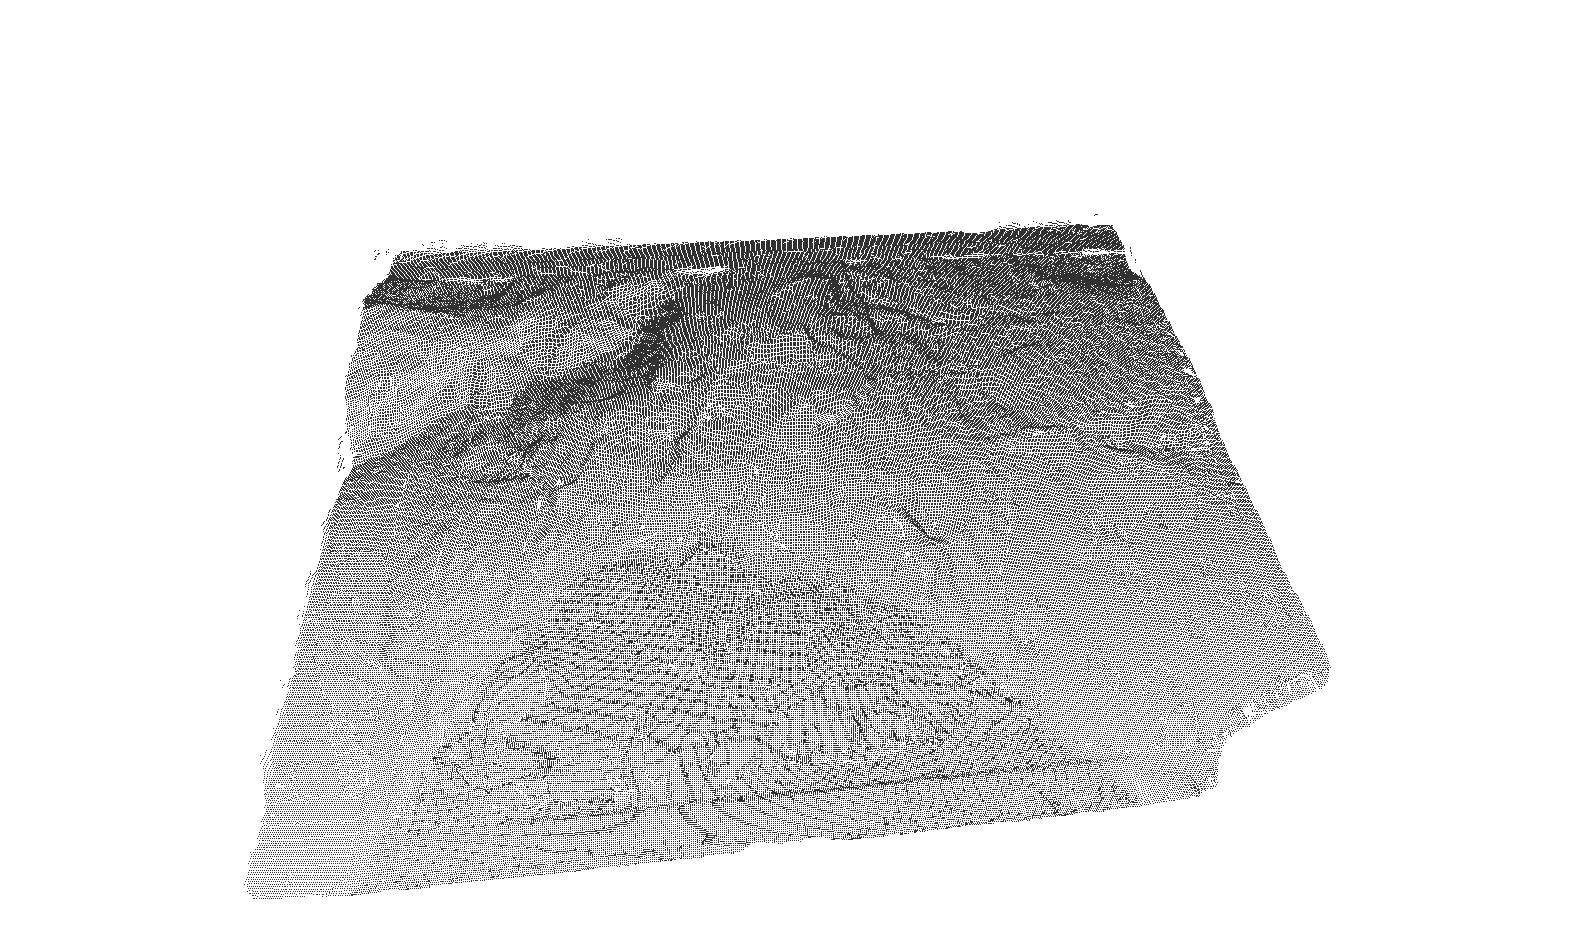
\includegraphics[width=0.6\textwidth]{./figures/MEX3-2PointCloud.png}
\end{center}
\caption{Point cloud representing the surface of a basalt sample from Thuringia. The size is 196 mm by 149 mm and the cloud contains approx. 252000 points.}
\label{fig:DataCNSBasaltPointCloud}
\end{figure}

\begin{figure}[!ht]
\begin{tabular}{cc}
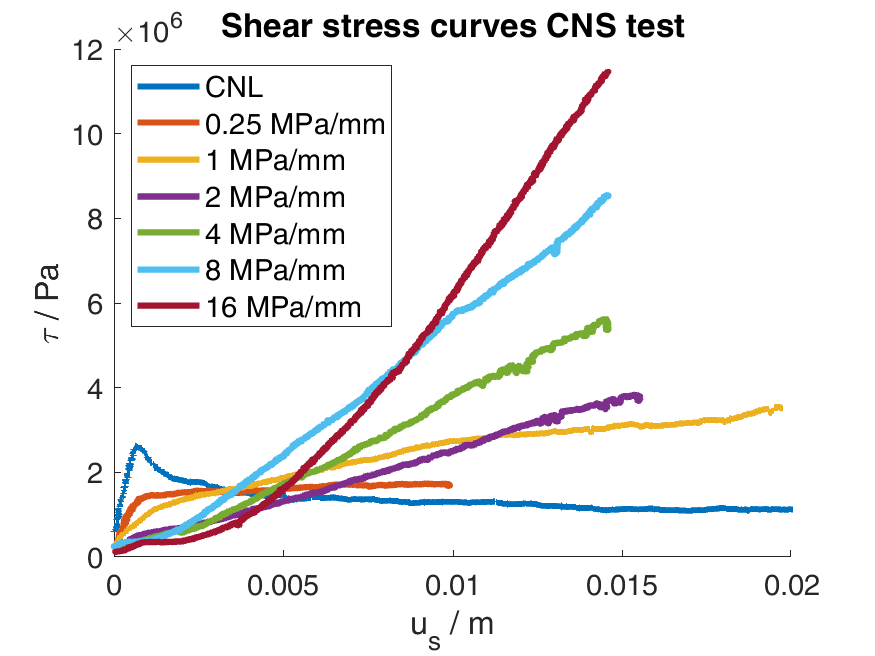
\includegraphics[width=0.45\textwidth]{./figures/CNSShearCurvesAll.png}     
& 
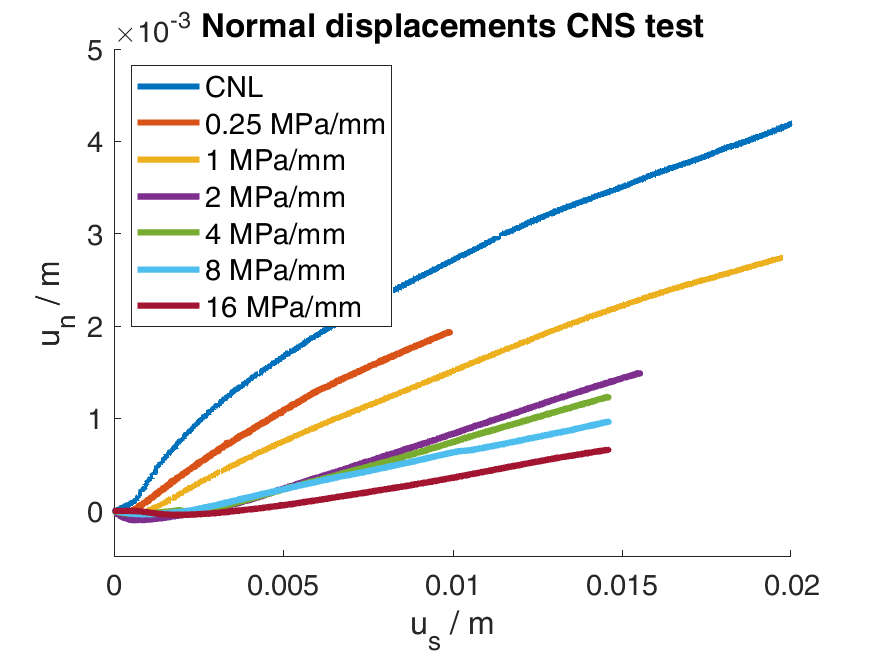
\includegraphics[width=0.45\textwidth]{./figures/CNSDilatationAll.png} 
\end{tabular}
\caption{CNS test results}
\label{fig:DataCNSBasaltLab}
\end{figure}

%---------------------------------------------------------
\subsubsection*{Meta Data Overview (according to Dublin Core)}
%---------------------------------------------------------

\begin{table}[!ht]
\caption{MEX 3-2 (TUBAF)}
\label{tab:dms-mex3-2}
\small
\begin{tabular}{R{3cm}|L{7cm}}
\hline
%
Data label & GeomInt, MEX 3-2, TUBAF, Data Set CNS \\
URI & http://www.ufz.de/record/dmp/archive/7924 \\
Subject  & Crystalline rock, direct shear test \\
Type of data  & collection of various data \\
Dataquality  & quality assured data \\
Status of data  & processed data \\
Dataformat  & txt, jpg, png \\
Creators  & TU Freiberg, Institut für Geotechnik, Gustav-Zeuner-Str. 1, 09599 Freiberg \\
Source/Origin  & Rock mechanical laboratory \\
Publisher  & TU Freiberg, Institut für Geotechnik, Gustav-Zeuner-Str. 1, 09599 Freiberg \\
Rights holders  & TU Freiberg, Institut für Geotechnik, Gustav-Zeuner-Str. 1, 09599 Freiberg \\
Contributors  & TU Freiberg, Institut für Geotechnik, Thomas Fr\"uhwirt and Daniel P\"otschke \\
Time/period of creation  & 2018 - 2019 \\
Language of the content & English \\
Update policy  & Stored data will not be extended \\
Access permissions  & Limited access \\
%
\hline
\end{tabular}
\end{table}